%----------------------------------------------------------------------------
\chapter{Overview of the Approach}
%----------------------------------------------------------------------------
In this chapter, the various aspects of the proposed approach are detailed. In Section \ref{sec_methodology}, the application of this methodology from the users' point of view: how are they supposed to interact with the interactive automata learning framework and how can they utilize it to design reactive systems in a declarative way. Then, in Section \ref{sec_architecture}, the applied software architecture, software components, algorithms and data structures are presented in the following order: first, the components concerned with the automata learning algorithm, then those responsible for its interaction with the oracle, then the possible interactions of the oracle with the engineer.
%----------------------------------------------------------------------------
\section{Overview of the Methodology} \label{sec_methodology}
%----------------------------------------------------------------------------
\begin{figure}[!ht] 
	\centering
	\fbox{
		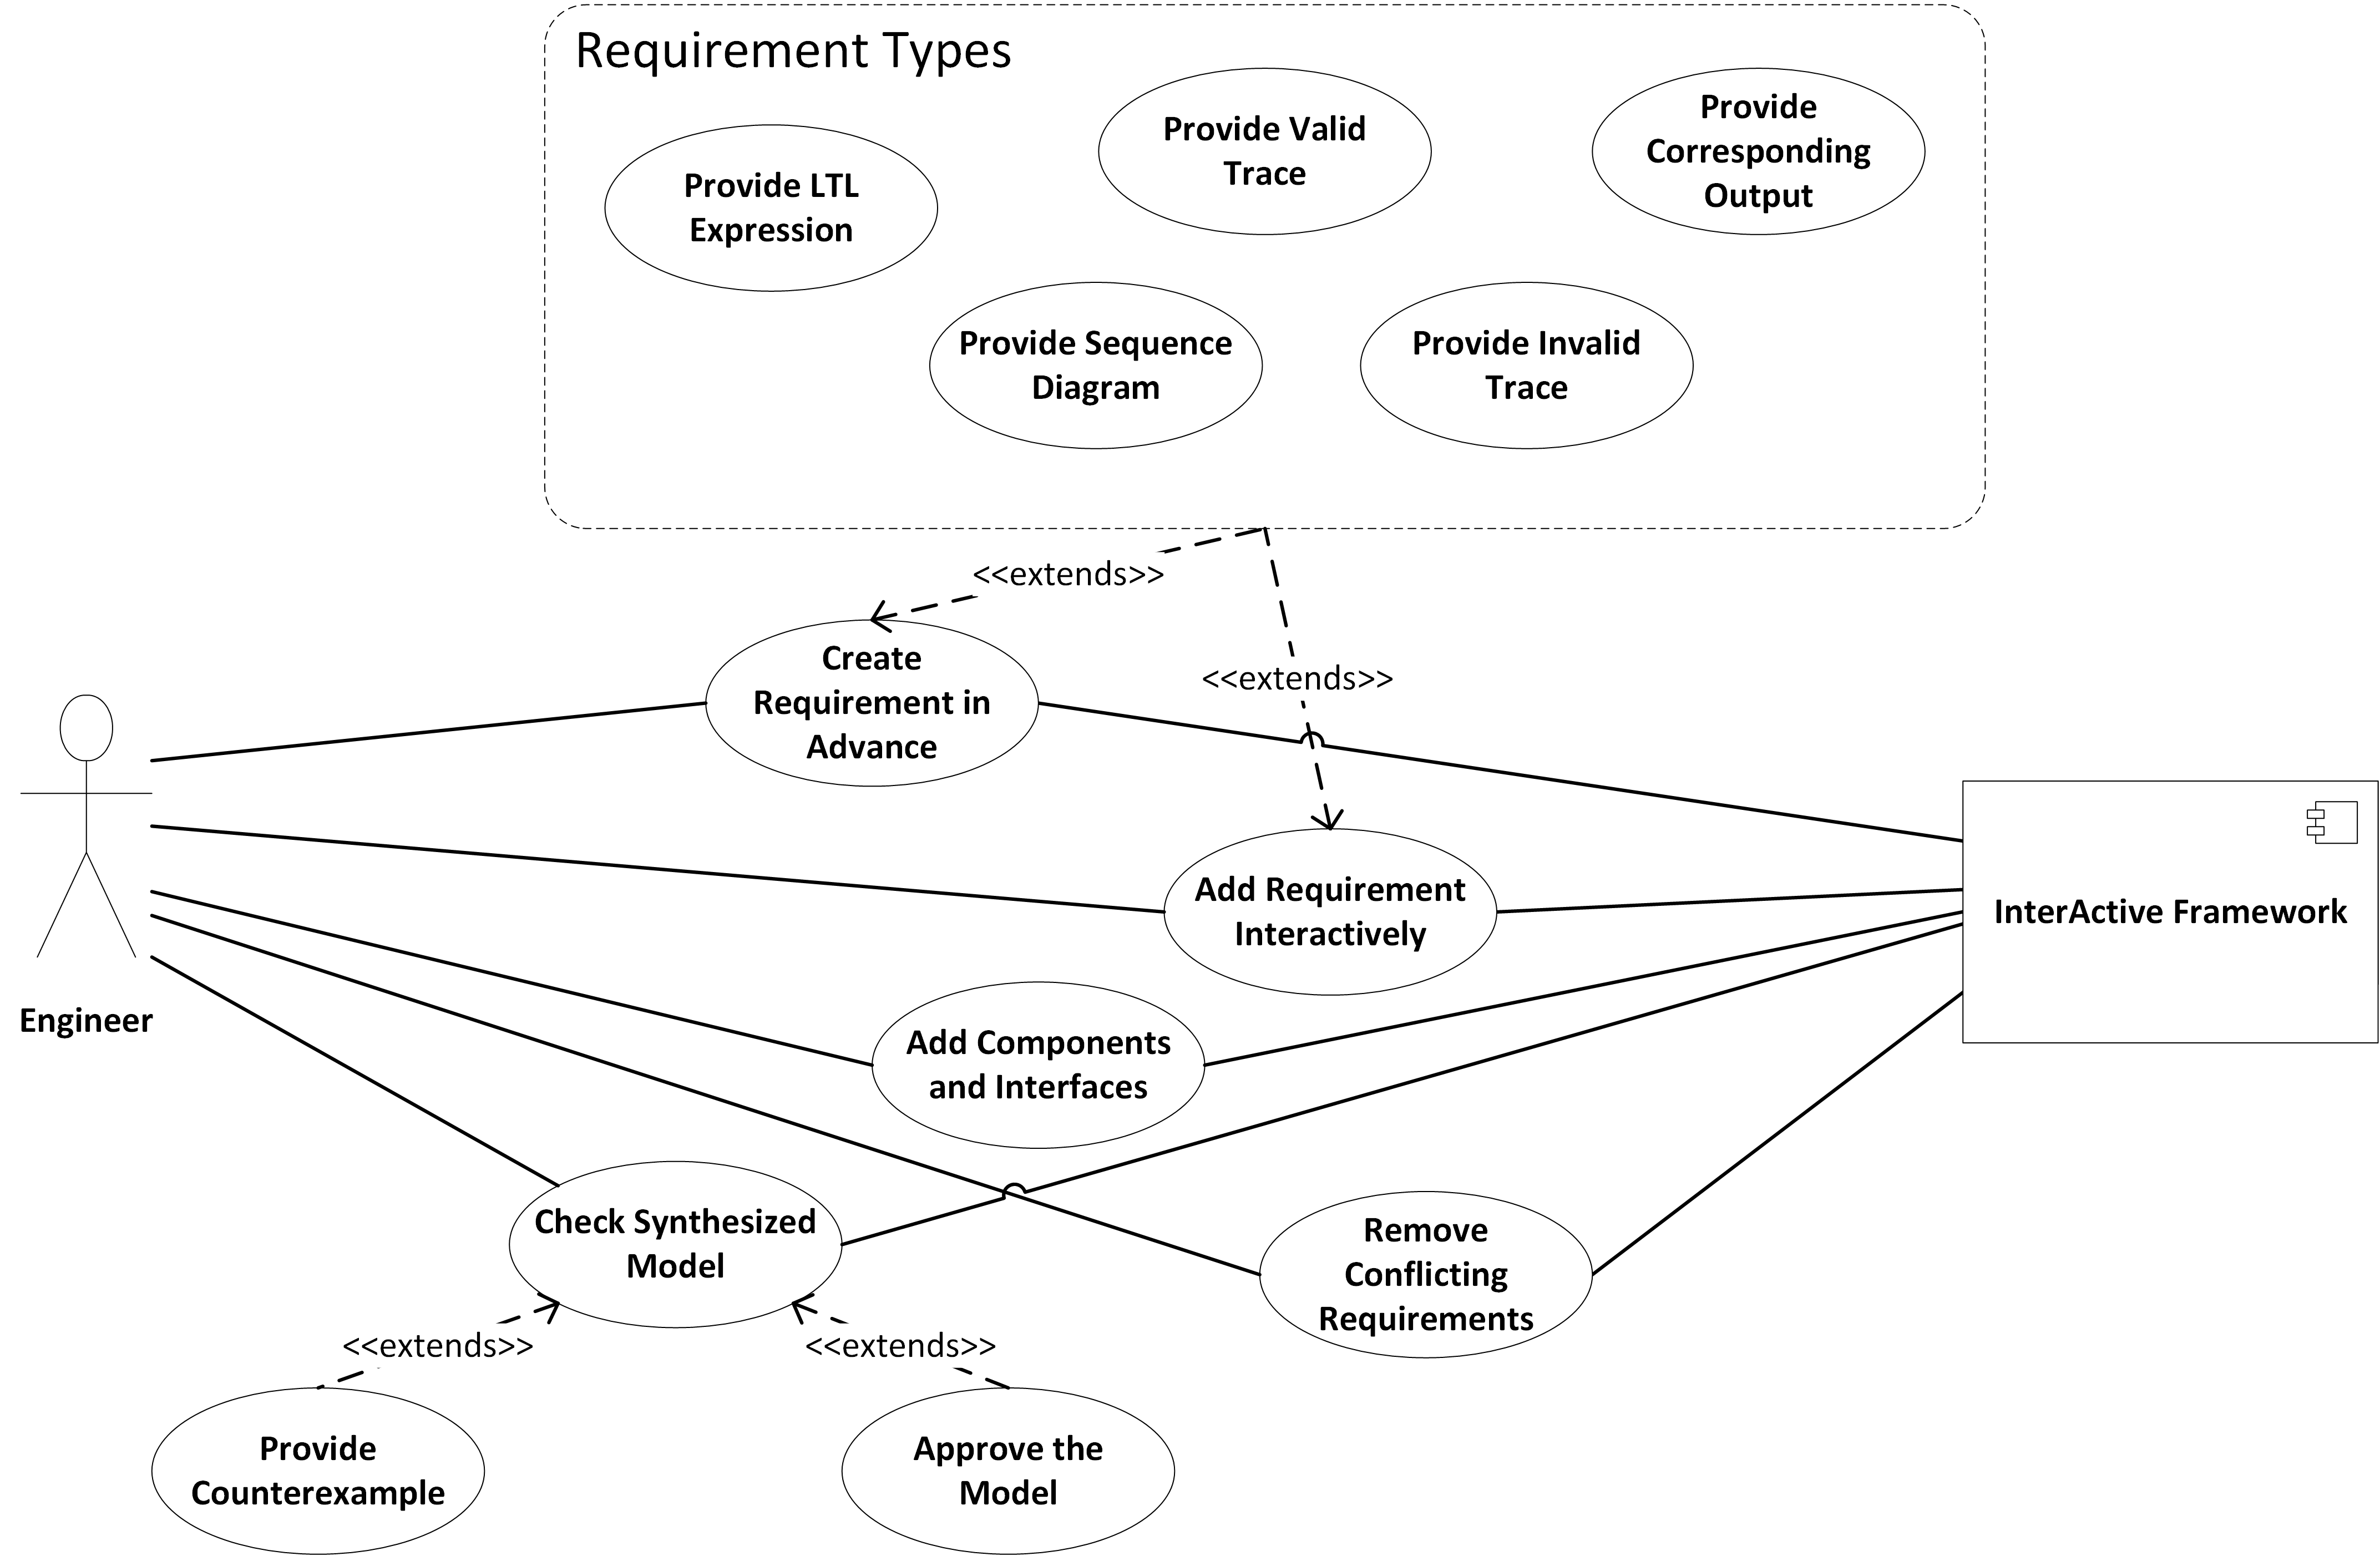
\includegraphics[width=150mm, keepaspectratio]{figures/methodology_interactiontypes.png}
	}
	\caption{Possibilities of the Engineer} %TODO title 
	\label{fig_methodology_interactiontypes}
\end{figure}

Our methodology is heavily based on the interaction of the user with the system, especially its \textit{Oracle} component. The different types of interaciton are summarized on Figure \ref{fig_methodology_interactiontypes} and elaborated on in Subsection \ref{subs_reqtypes}. These interactions take place in a predefined order - the \textit{proposed workflow}, illustrated on Figure \ref{fig_methodology_workflow}. This workflow consists of two phases: first, an \textit{offline} one, and then an \textit{online} one. During the offline phase, the system offers little assistance, the designing engineer must determine the required details by other means. The interactive system design happens during the online phase. 

The individual steps in both the offline and the online phases have a predefined syntax with the corresponding, precisely defined semantics. Their common feature is the declarative way of describing the system components, which allows the engineer to focus solely on the expected behavior and acquire a minimal model exhibiting the specified functionality. The following subsections explain these steps in detail.

\begin{figure}[!ht] 
	\centering
	\fbox{
		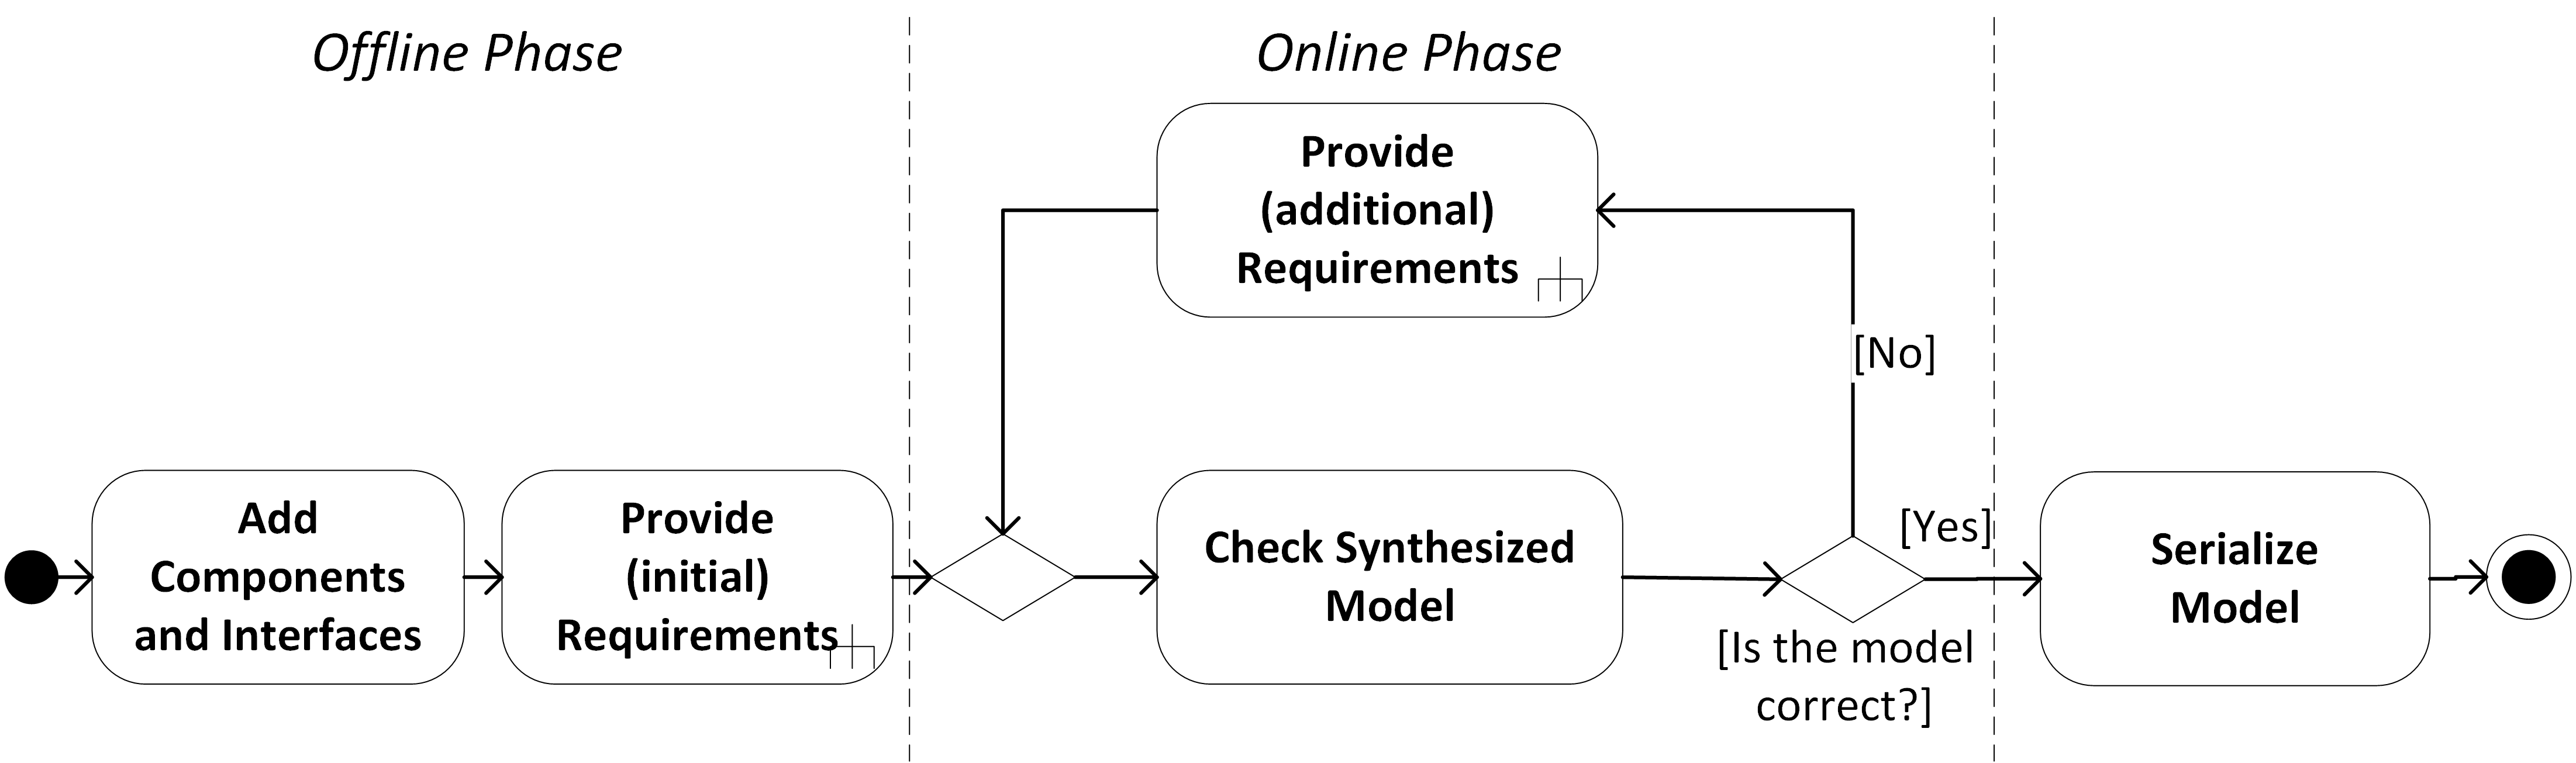
\includegraphics[width=150mm, keepaspectratio]{figures/methodology_workflow.png}
	}
	\caption{The Proposed Workflow} %TODO title 
	\label{fig_methodology_workflow}
\end{figure}
%TODO fork a komponenseknek
%TODO bekeretezni az online és az offline részeket, meg feliratozni

%---------------------------------------------------------------
\subsection{Component and Interface Definition} \label{subs_compdef}
%---------------------------------------------------------------
%TODO megadhat több komponenst, névvel, ezek a megfelelő viselkedéseket fogják tanúsítani. I/O ábécét megadjuk előre, komponensek kapcsolatát a nevekből inferáljuk. Mindegyiket TELJESEN KÜLÖN tanuljuk (fork). Ezért egyelőre semmit sem garantálunk ilyen téren, de előnyei is vannak.
The first step of the workflow is the declaration of the system components. This happens in the offline phase, as the determination of the system components, their exact boundaries and interfaces is out of the scope of this work. Nonetheless, the engineer must provide the names of the system components, along with their input- and output alphabets, before the workflow can proceed to the next step.

Users are encouraged to specify input and output characters qualified with port names in the format 'Port.character', as this supplies the subsequent steps with essential information about the connections of the individual system components.

The components are handled as independent systems in every other aspect. This results - among others - in the arbitrary ordering of the online behavior-learning phases, and the behavioral faults being limited to their components of origin (although this does not limit the propagation of errors through messages resulting from incorrect behavior).

The syntax of component and interface definitions is quite simple, as illustrated in [TODO add example]

%---------------------------------------------------------------
\subsection{Requirement Types} \label{subs_reqtypes}
%---------------------------------------------------------------
% Mi a szintaxis (LTL: syntactic constructs, operátor precedencia, szemandtika - hivatkozások a megfelelő cikkre)
% Mi a szemantika (LTL->LTS alapú def ref background)
During the workflow, the engineers can provide the requirements in both the online and the offline phases. 

In the offline phase, this means that they add requirements they have formulated in advance. This is useful for more general requirements, with the scope of the whole component, conveniently formulated by program logic expressions, or long and complex traces.

In the online phase, adding requirements means answering the questions formulated by the algorithm, about a yet unknown behavior at a specific place in the currently examined trace. This too can be answered through program logic - e.g. when the engineer realizes a general property during the model construction - but also through traces and through giving the corresponding output directly.

\textbf{Corresponding Output}
% TODO ref background: trace(-based)

This is the simplest way of specifying the behavior of the system, also containing the least information among the different model types. To put simply, this means giving the output for a given input sequence, without any additional information. This supposedly answers the question of the <system> at \textit{one} given point, and that is the end of its scope.

An example can be seen on [TODO insert example]

\textbf{Valid Trace}

Valid traces are the more complex form of giving the corresponding output: it gives the corresponding output for any prefix of the contained input sequence. This might be useful, as usually the whole output sequence is taken into consideration when determining the output for some inputs. Thus, the <system> can get \textit{multiple} answers concerning the behavior in question.

An example can be seen on [TODO insert example]

\textbf{Sequence Diagram}
%TODO ref backgr UML

UML-like sequence diagrams are an even more complex form of trace-based models, as they can contain several traces - due to them having \textit{alt} and \textit{opt} fragments for branching the behavior. They also have - among others - \textit{ref} fragments for referencing behaviors specified elsewhere.

Sequence diagrams can also be used to model infinite behavior, which results in containing plenty of information, which in turn results in possibly answering \textit{several} questions formulated by the <system>.

An example for the application of sequence diagrams can be seen on [TODO insert example]

It is important to note, that the specification and integration of sequence diagrams into this framework is not yet complete. 

\textbf{Trace to Exclude}

Invalid traces are similar to valid traces, with the difference that the contained behavior must not appear in the resulting model. 

They are most useful for small output alphabets, or when the range of possible behaviors is otherwise contained - e.g. through program logic expressions or several other excluded traces.

They can also be used to formulate requirements even when the determination of the correct behavior does not directly follow from these models: the <system> will signal conflicting requirements for the examined input sequences and require the user to remove one.

An example can be seen on [TODO insert example]

\textbf{LTL Expression}
%TODO ref backgr LTL
%TODO ref backgr LTS

LTL expressions are a highly complex type of program logic-based requirement specification: they can be used to formulate propositional logic expressions with temporal connectives over \textit{paths} of a \textit{base model}, as described in [TODO backgr]. For our application, we introduce our own LTL expression language with its own syntax and semantics - although attempting to keep it similar to other generally known variants, especially that of SPOT [TODO ref].
%In our case, the LTS interpretation of the system under learning will serve as the base model, and the expression has to be valid over all paths from the initial state.  
%TODO has to be valid or has to be able to be valid???
The syntax of the LTL expressions is as follows:
...
...

The base model will be ... [TODO backgr LTS]
In our interpretation, the LTL expressions must hold for all paths from the initial state.

The semantics of the supported temporal connectives are similar to those described in [TODO ref] %TODO ref backgr

An example for a valid LTL expression can be seen on [TODO insert example]

It is important to note, that the specification of our LTL variant is not yet complete: for the compactness of requirement specifications it would make sense to integrate additional well-known boolean operators - like XOR (exclusive-or) - and temportal connectives - like WB (weak-before) and R (release) - into the language. 

%---------------------------------------------------------------
\subsection{Conflicting Requirements} \label{subs_conf}
%---------------------------------------------------------------
%TODO konfliktusban álló követelményeket mikor tud kivenni
% Diszjunktság nehéz kérdés (ref Backgr), csak akkor dobjuk fel, ha valami bemenetre gond van
% Akkor kiveheti az egyiket
% Konzisztenciát többé-kevésbé figyeljük

%---------------------------------------------------------------
\subsection{Equivalence Query} \label{subs_eq}
%---------------------------------------------------------------
%TODO megjeleníti az EQt, mi van ekkor
% Ha tetszik, elfogadjuk és továbblép a workflowban
% Ha nem tetszik, adunk egy ellenpélda-input-sorozatot
% TULAJDONSÁGAI?
%---------------------------------------------------------------
\subsection{The Resulting Model} \label{subs_resultingmodel}
%---------------------------------------------------------------
%TODO ha minden kész, valid Gammát kapunk, ezt:
% kiegészíthetjük
% generálhatunk belőle akármit, amit a gamma tud (ref backgr)

%----------------------------------------------------------------------------
\section{Overview of the Architecture} \label{sec_architecture}
%----------------------------------------------------------------------------